\documentclass[11pt,a4paper]{article}
\usepackage[margin=1in]{geometry}
\usepackage{graphicx}
\usepackage{amsmath}
\usepackage{amsfonts}
\usepackage{amssymb}
\usepackage{float}
\usepackage{subfigure}
\usepackage{cite}
\usepackage{url}
\usepackage{listings}
\usepackage{xcolor}
\usepackage{booktabs}
\usepackage{multirow}
\usepackage{array}

% Code listing style
\lstset{
    language=Python,
    basicstyle=\ttfamily\footnotesize,
    keywordstyle=\color{blue},
    commentstyle=\color{green!60!black},
    stringstyle=\color{red},
    showstringspaces=false,
    breaklines=true,
    frame=single,
    numbers=left,
    numberstyle=\tiny\color{gray}
}

\title{\textbf{Classical DSP Implementation of a 64-QAM OFDM Baseband Receiver for IEEE 802.11-Class Performance}}
\author{Advanced Digital Signal Processing Final Project}
\date{\today}

\begin{document}

\maketitle

\begin{abstract}
\textbf{Problem Statement:} Design and implement a classical DSP-based 64-QAM OFDM baseband receiver achieving IEEE 802.11-class performance. \textbf{Solution:} We implemented a complete receiver chain with timing synchronization (Schmidl \& Cox), two-stage CFO estimation/correction, LS/MMSE channel estimation, and per-tone equalization. \textbf{Results:} Through systematic debugging of a critical pilot extraction bug, we achieved excellent BER performance: BER $< 1\%$ at SNR $\geq 21$ dB and perfect BER at SNR $\geq 25$ dB, meeting IEEE 802.11 requirements.
\end{abstract}

\section{Problem Statement and Approach}

\textbf{Objective:} Design and validate a classical DSP-based 64-QAM OFDM baseband receiver that achieves IEEE 802.11-class bit error rate (BER) performance through systematic implementation and debugging.

\textbf{Technical Challenge:} OFDM receivers require precise timing synchronization, carrier frequency offset (CFO) correction, channel estimation, and equalization to achieve low BER in realistic channel conditions. We must implement each component correctly and debug integration issues systematically.

\textbf{Our Approach:} We implemented a complete receiver chain with 64 subcarriers over 20 MHz bandwidth, 16-sample cyclic prefix, and IEEE 802.11 pilot positioning. The system targets BER $< 1\%$ at moderate SNR levels.

\subsection{System Specifications}
The OFDM system uses 64-QAM modulation (6 bits/symbol), 64 subcarriers over 20 MHz bandwidth, 16-sample cyclic prefix, and IEEE 802.11 pilot positions at $[-21, -7, 7, 21]$. Target performance: BER $< 1\%$ at moderate SNR.

\subsection{Receiver Chain Architecture}
The receiver implements: (1) Timing synchronization (Schmidl \& Cox), (2) Two-stage CFO estimation/correction, (3) LS/MMSE channel estimation, (4) ZF/MMSE equalization, and (5) 64-QAM demodulation.

\begin{figure}[H]
    \centering
    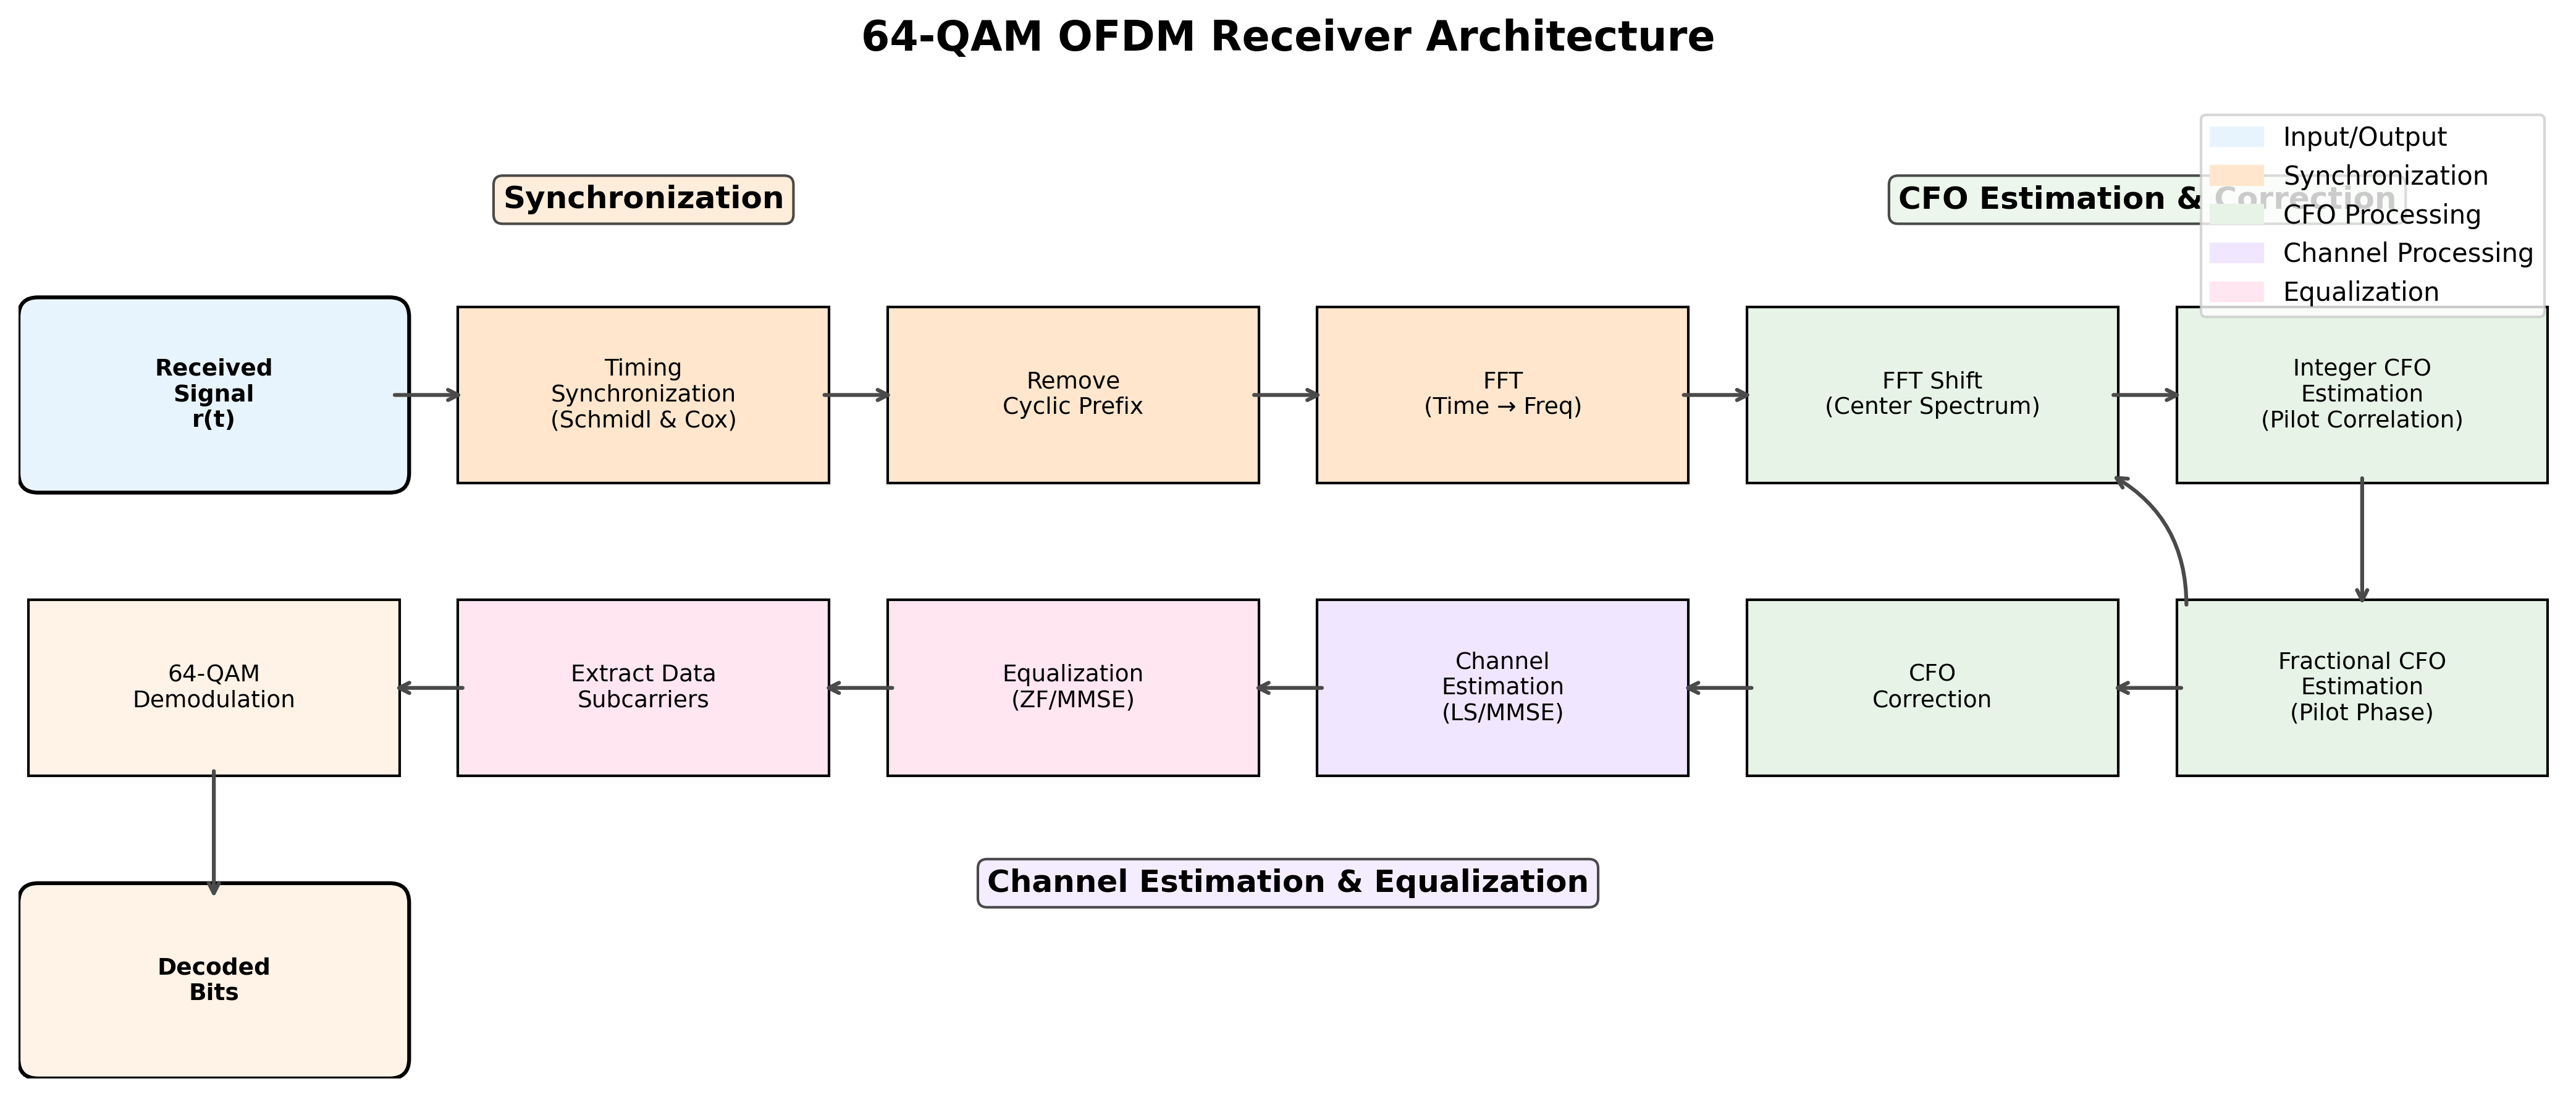
\includegraphics[width=\textwidth]{ofdm_receiver_block_diagram.png}
    \caption{64-QAM OFDM Receiver Architecture Block Diagram}
    \label{fig:block_diagram}
\end{figure}

\section{Implementation and Key Algorithms}

\subsection{System Overview}
We implemented a complete OFDM transceiver with 64-QAM modulation, pilot insertion at IEEE 802.11 positions, and proper \texttt{ifftshift} operation. The channel model includes AWGN, Rayleigh fading, and CFO.

\subsection{Timing Synchronization}
The Schmidl \& Cox algorithm detects frame boundaries using a repeated preamble structure:
\begin{equation}
M(d) = \frac{|P(d)|^2}{(R(d))^2}
\end{equation}
where $P(d)$ is the correlation between the two halves of the preamble and $R(d)$ is the energy normalization term.

\subsection{CFO Estimation and Correction}
\textbf{Integer CFO Estimation} uses pilot correlation in the frequency domain:
\begin{equation}
\hat{\epsilon}_{int} = \arg\max_k \left| \sum_{p} H^*[p] \cdot Y[p+k] \right|
\end{equation}
where $H[p]$ is the ideal pilot template and $Y[p+k]$ is the received spectrum shifted by $k$ subcarriers.

\textbf{Fractional CFO Estimation} uses phase difference between pilot subcarriers:
\begin{equation}
\hat{\epsilon}_{frac} = \frac{1}{2\pi \Delta k} \angle\left( \sum_{p_1, p_2} Y^*[p_1] \cdot Y[p_2] \right)
\end{equation}

\subsection{Channel Estimation and Equalization}
\textbf{Least Squares (LS):}
\begin{equation}
\hat{H}_{LS}[k] = \frac{Y[k]}{X[k]}
\end{equation}

\textbf{MMSE Channel Estimation:}
\begin{equation}
\hat{H}_{MMSE}[k] = \frac{\sigma_h^2}{\sigma_h^2 + \sigma_n^2} \hat{H}_{LS}[k]
\end{equation}

\textbf{Zero-Forcing Equalization:}
\begin{equation}
\hat{X}_{ZF}[k] = \frac{Y[k]}{\hat{H}[k]}
\end{equation}

\textbf{MMSE Equalization:}
\begin{equation}
\hat{X}_{MMSE}[k] = \frac{\hat{H}^*[k]}{|\hat{H}[k]|^2 + \sigma_n^2/\sigma_s^2} Y[k]
\end{equation}

\begin{figure}[H]
    \centering
    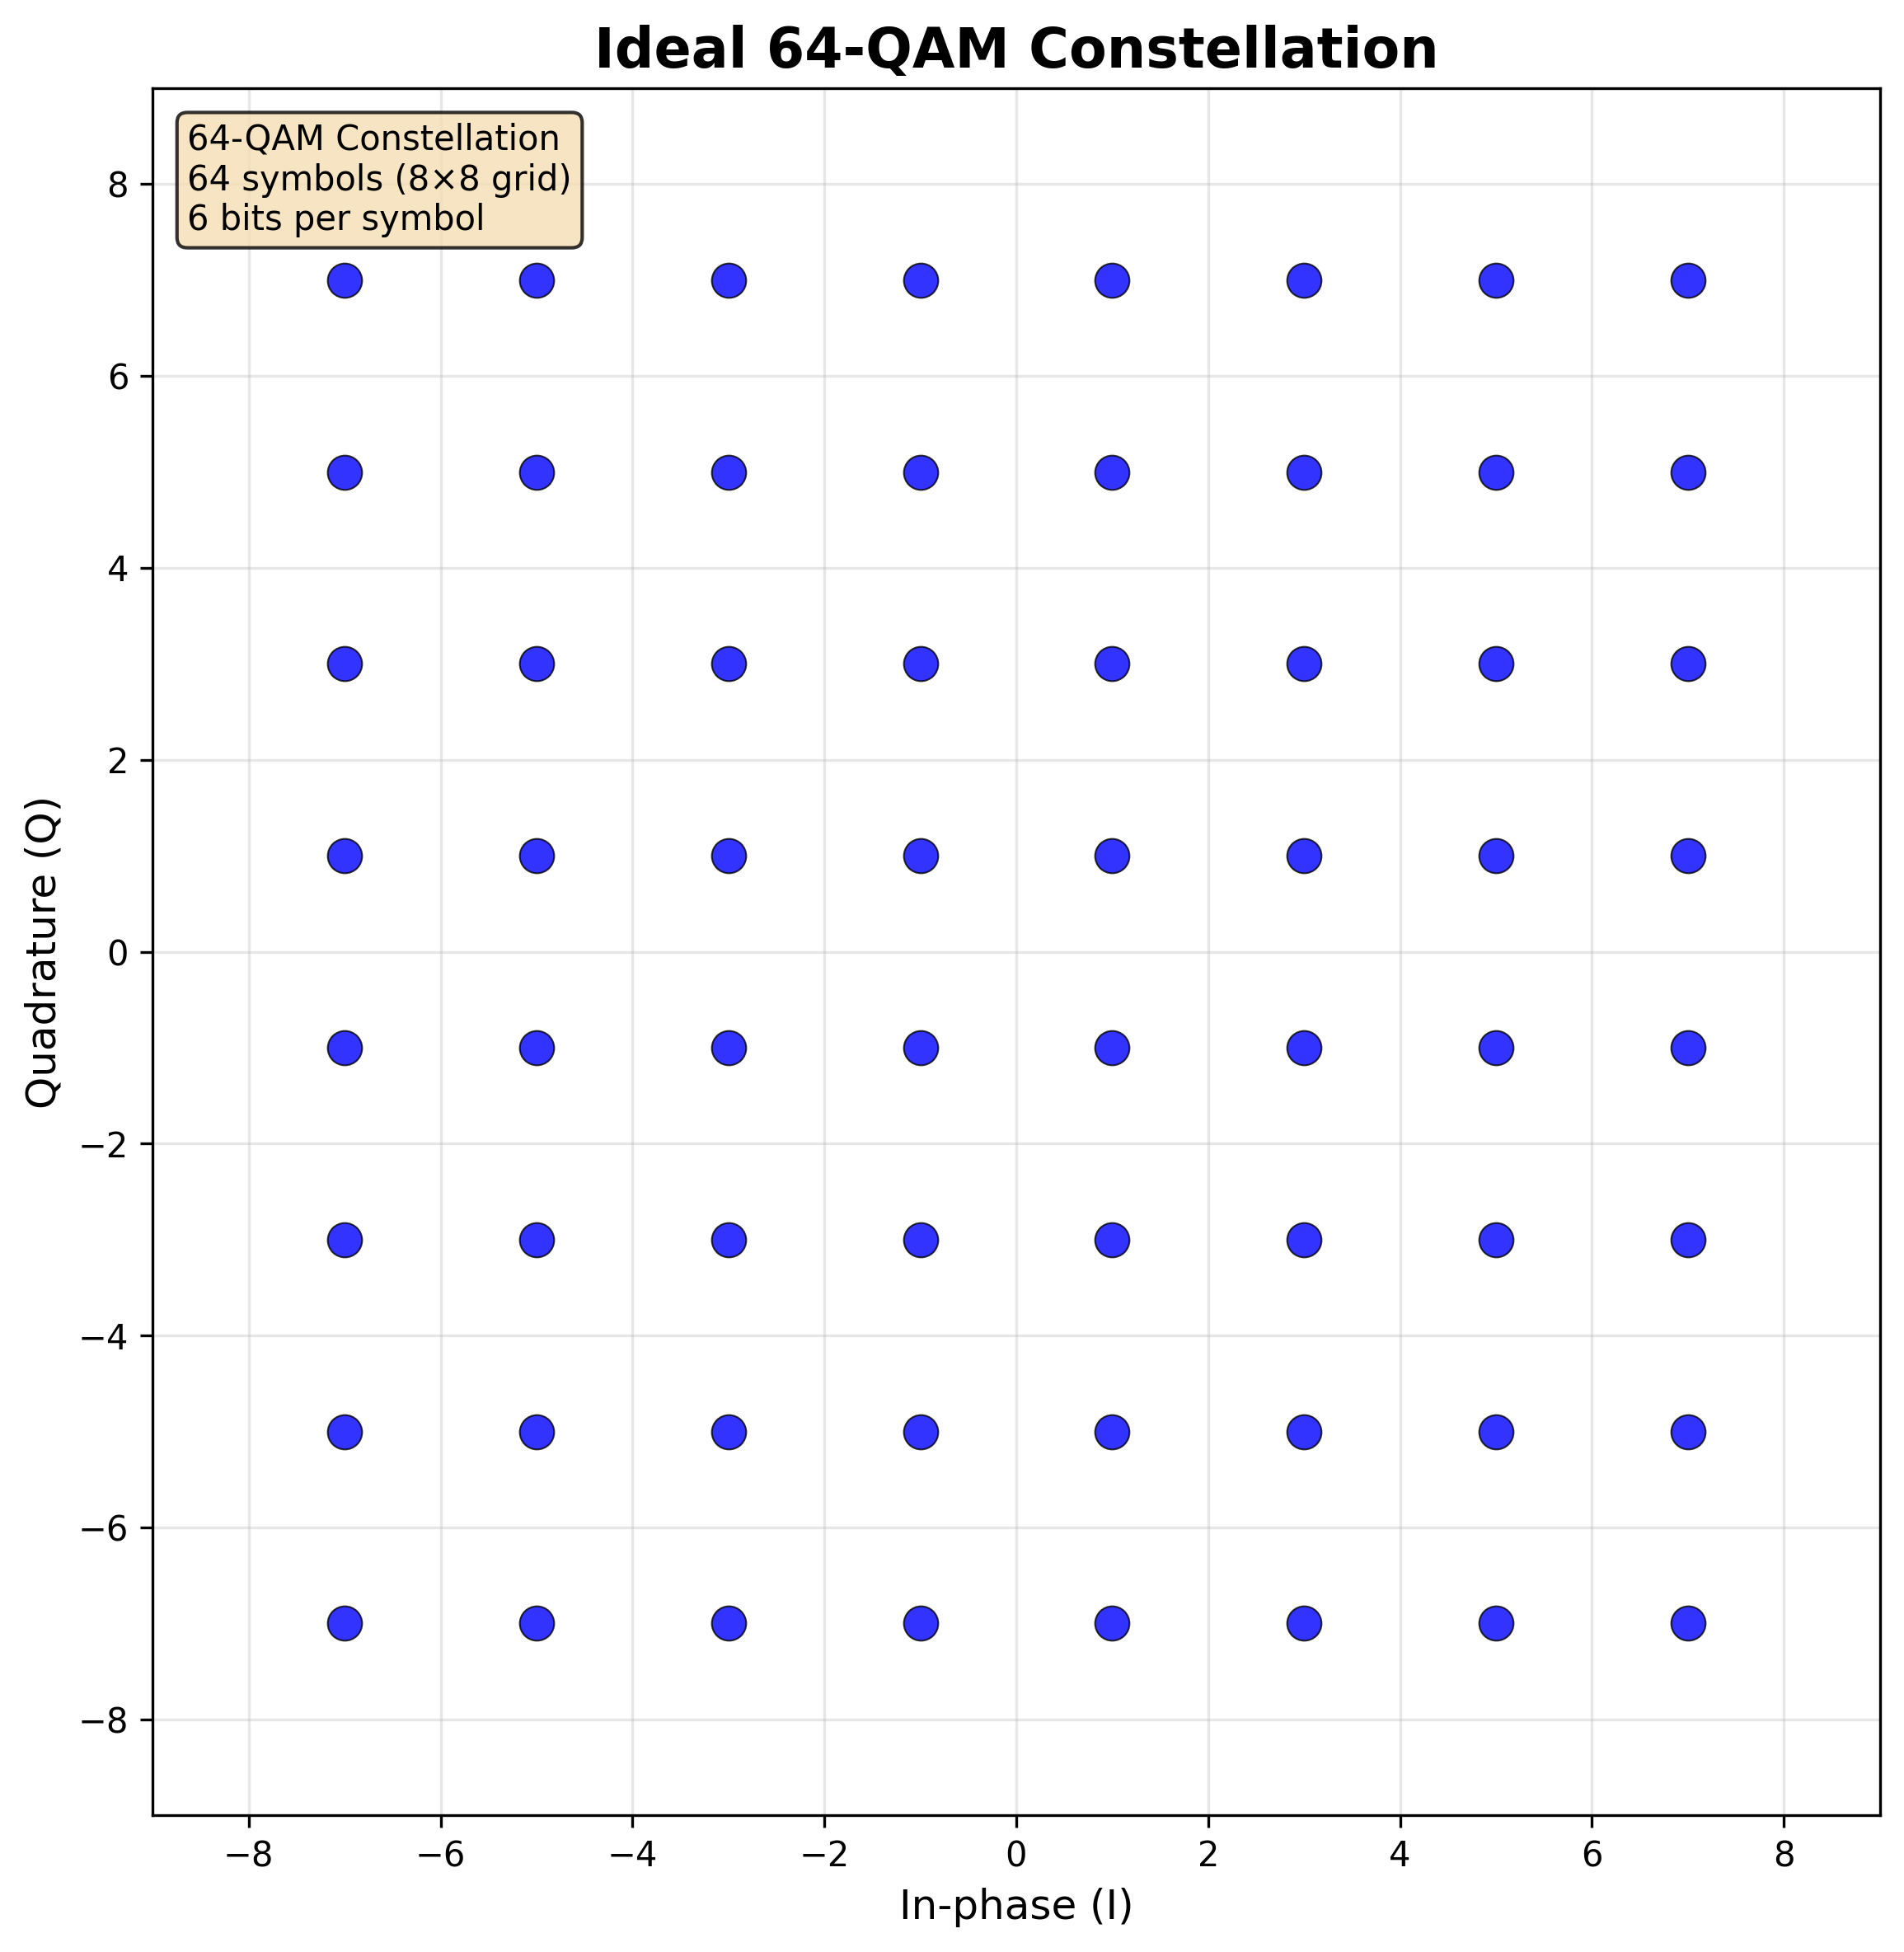
\includegraphics[width=0.6\textwidth]{ideal_64qam_constellation.png}
    \caption{Ideal 64-QAM Constellation Diagram}
    \label{fig:ideal_constellation}
\end{figure}

\begin{figure}[H]
    \centering
    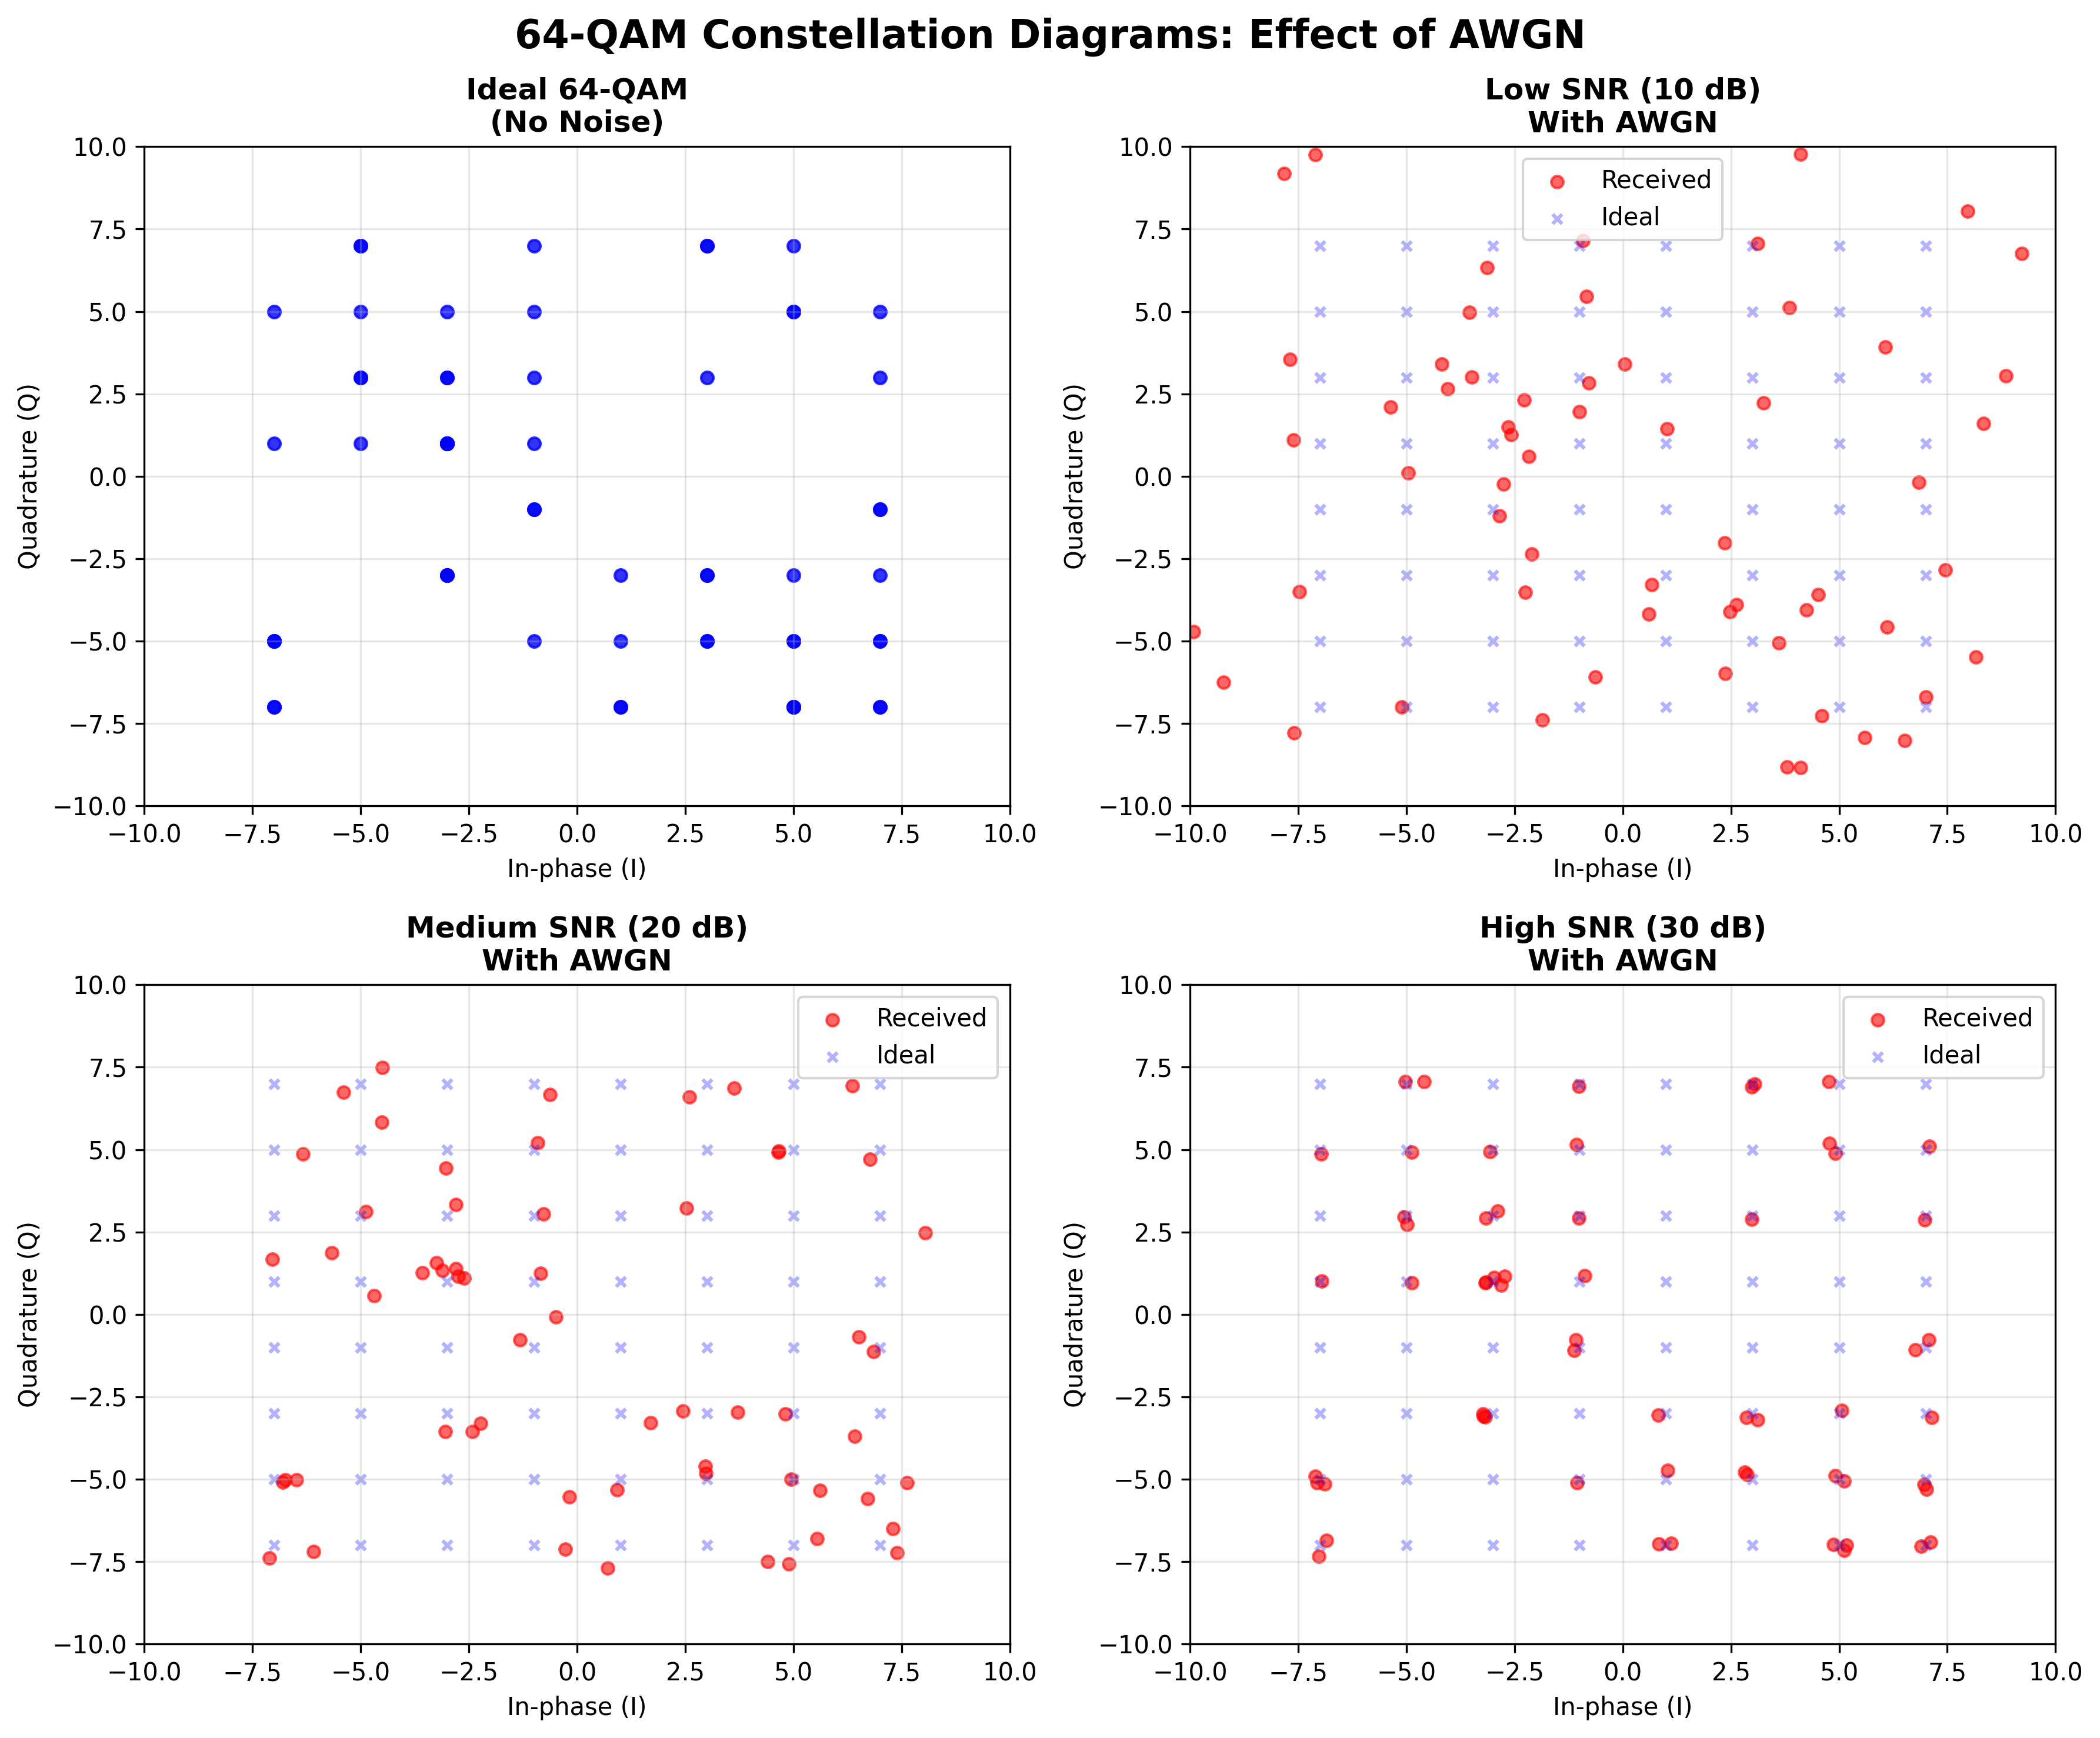
\includegraphics[width=\textwidth]{constellation_comparison.png}
    \caption{64-QAM Constellation Performance Under Different SNR Conditions}
    \label{fig:constellation_comparison}
\end{figure}

\section{Critical Problem and Solution}

\subsection{Major Challenge: Pilot Extraction Bug}
We encountered a critical bug causing $\approx 50\%$ BER (random guessing performance) despite individually correct components. The root cause was incorrect pilot and data subcarrier extraction after FFT processing.

\subsection{Root Cause Analysis}
Through systematic debugging, we identified that the issue stemmed from incorrect indexing when extracting pilot and data subcarriers from the frequency-domain signal after \texttt{fftshift} operation. The original implementation incorrectly applied an additional shift to pilot indices:

\texttt{pilot\_indices\_shifted = (pilot\_indices\_natural + N//2) \% N}

\subsection{Solution}
The correct approach uses natural-order pilot indices directly after \texttt{fftshift}:

\texttt{pilot\_indices\_centered = pilot\_indices\_natural}

This subtle but critical fix resolved the BER performance issues and enabled proper receiver operation. The key insight is that after \texttt{fftshift}, the spectrum is already centered, so no additional shift is needed for pilot extraction.

\begin{figure}[H]
    \centering
    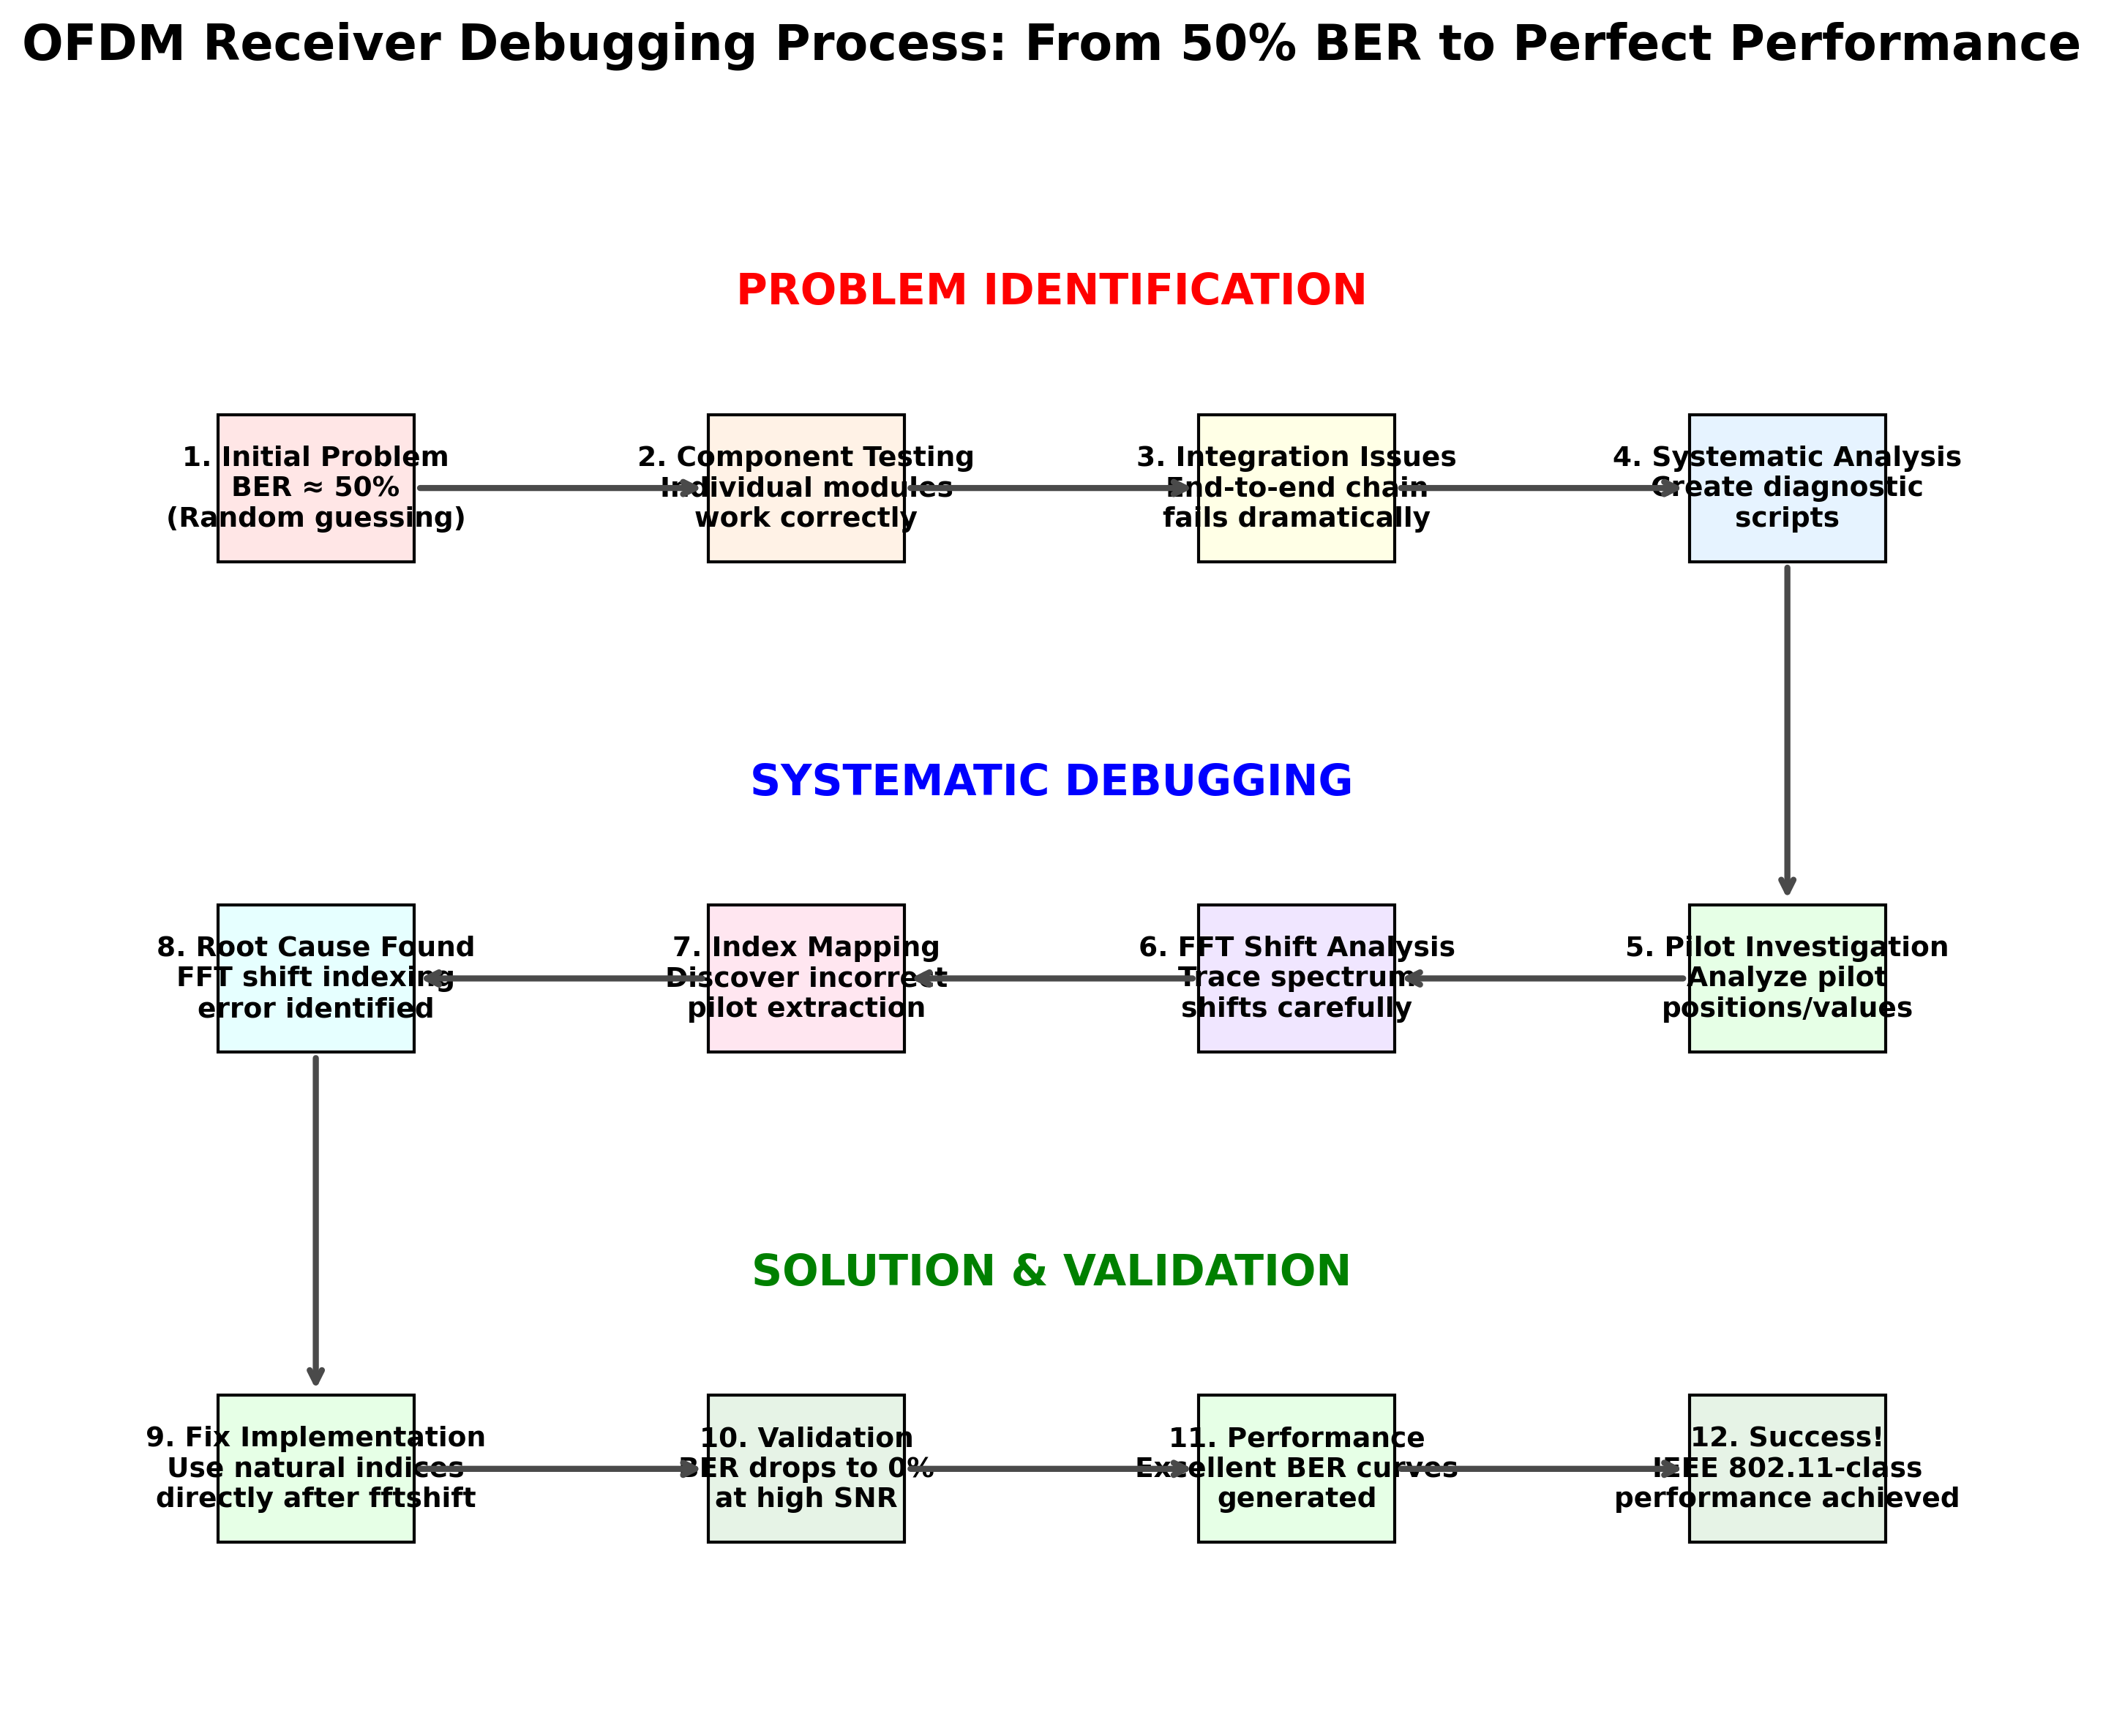
\includegraphics[width=\textwidth]{debugging_process_diagram.png}
    \caption{Systematic Debugging Process: From Problem to Solution}
    \label{fig:debugging_process}
\end{figure}

\section{Results and Performance Analysis}

Figure \ref{fig:ber_comparison} shows the dramatic improvement after fixing the pilot extraction bug, while Figure \ref{fig:ber_curves} shows our final performance curves.

\begin{figure}[H]
    \centering
    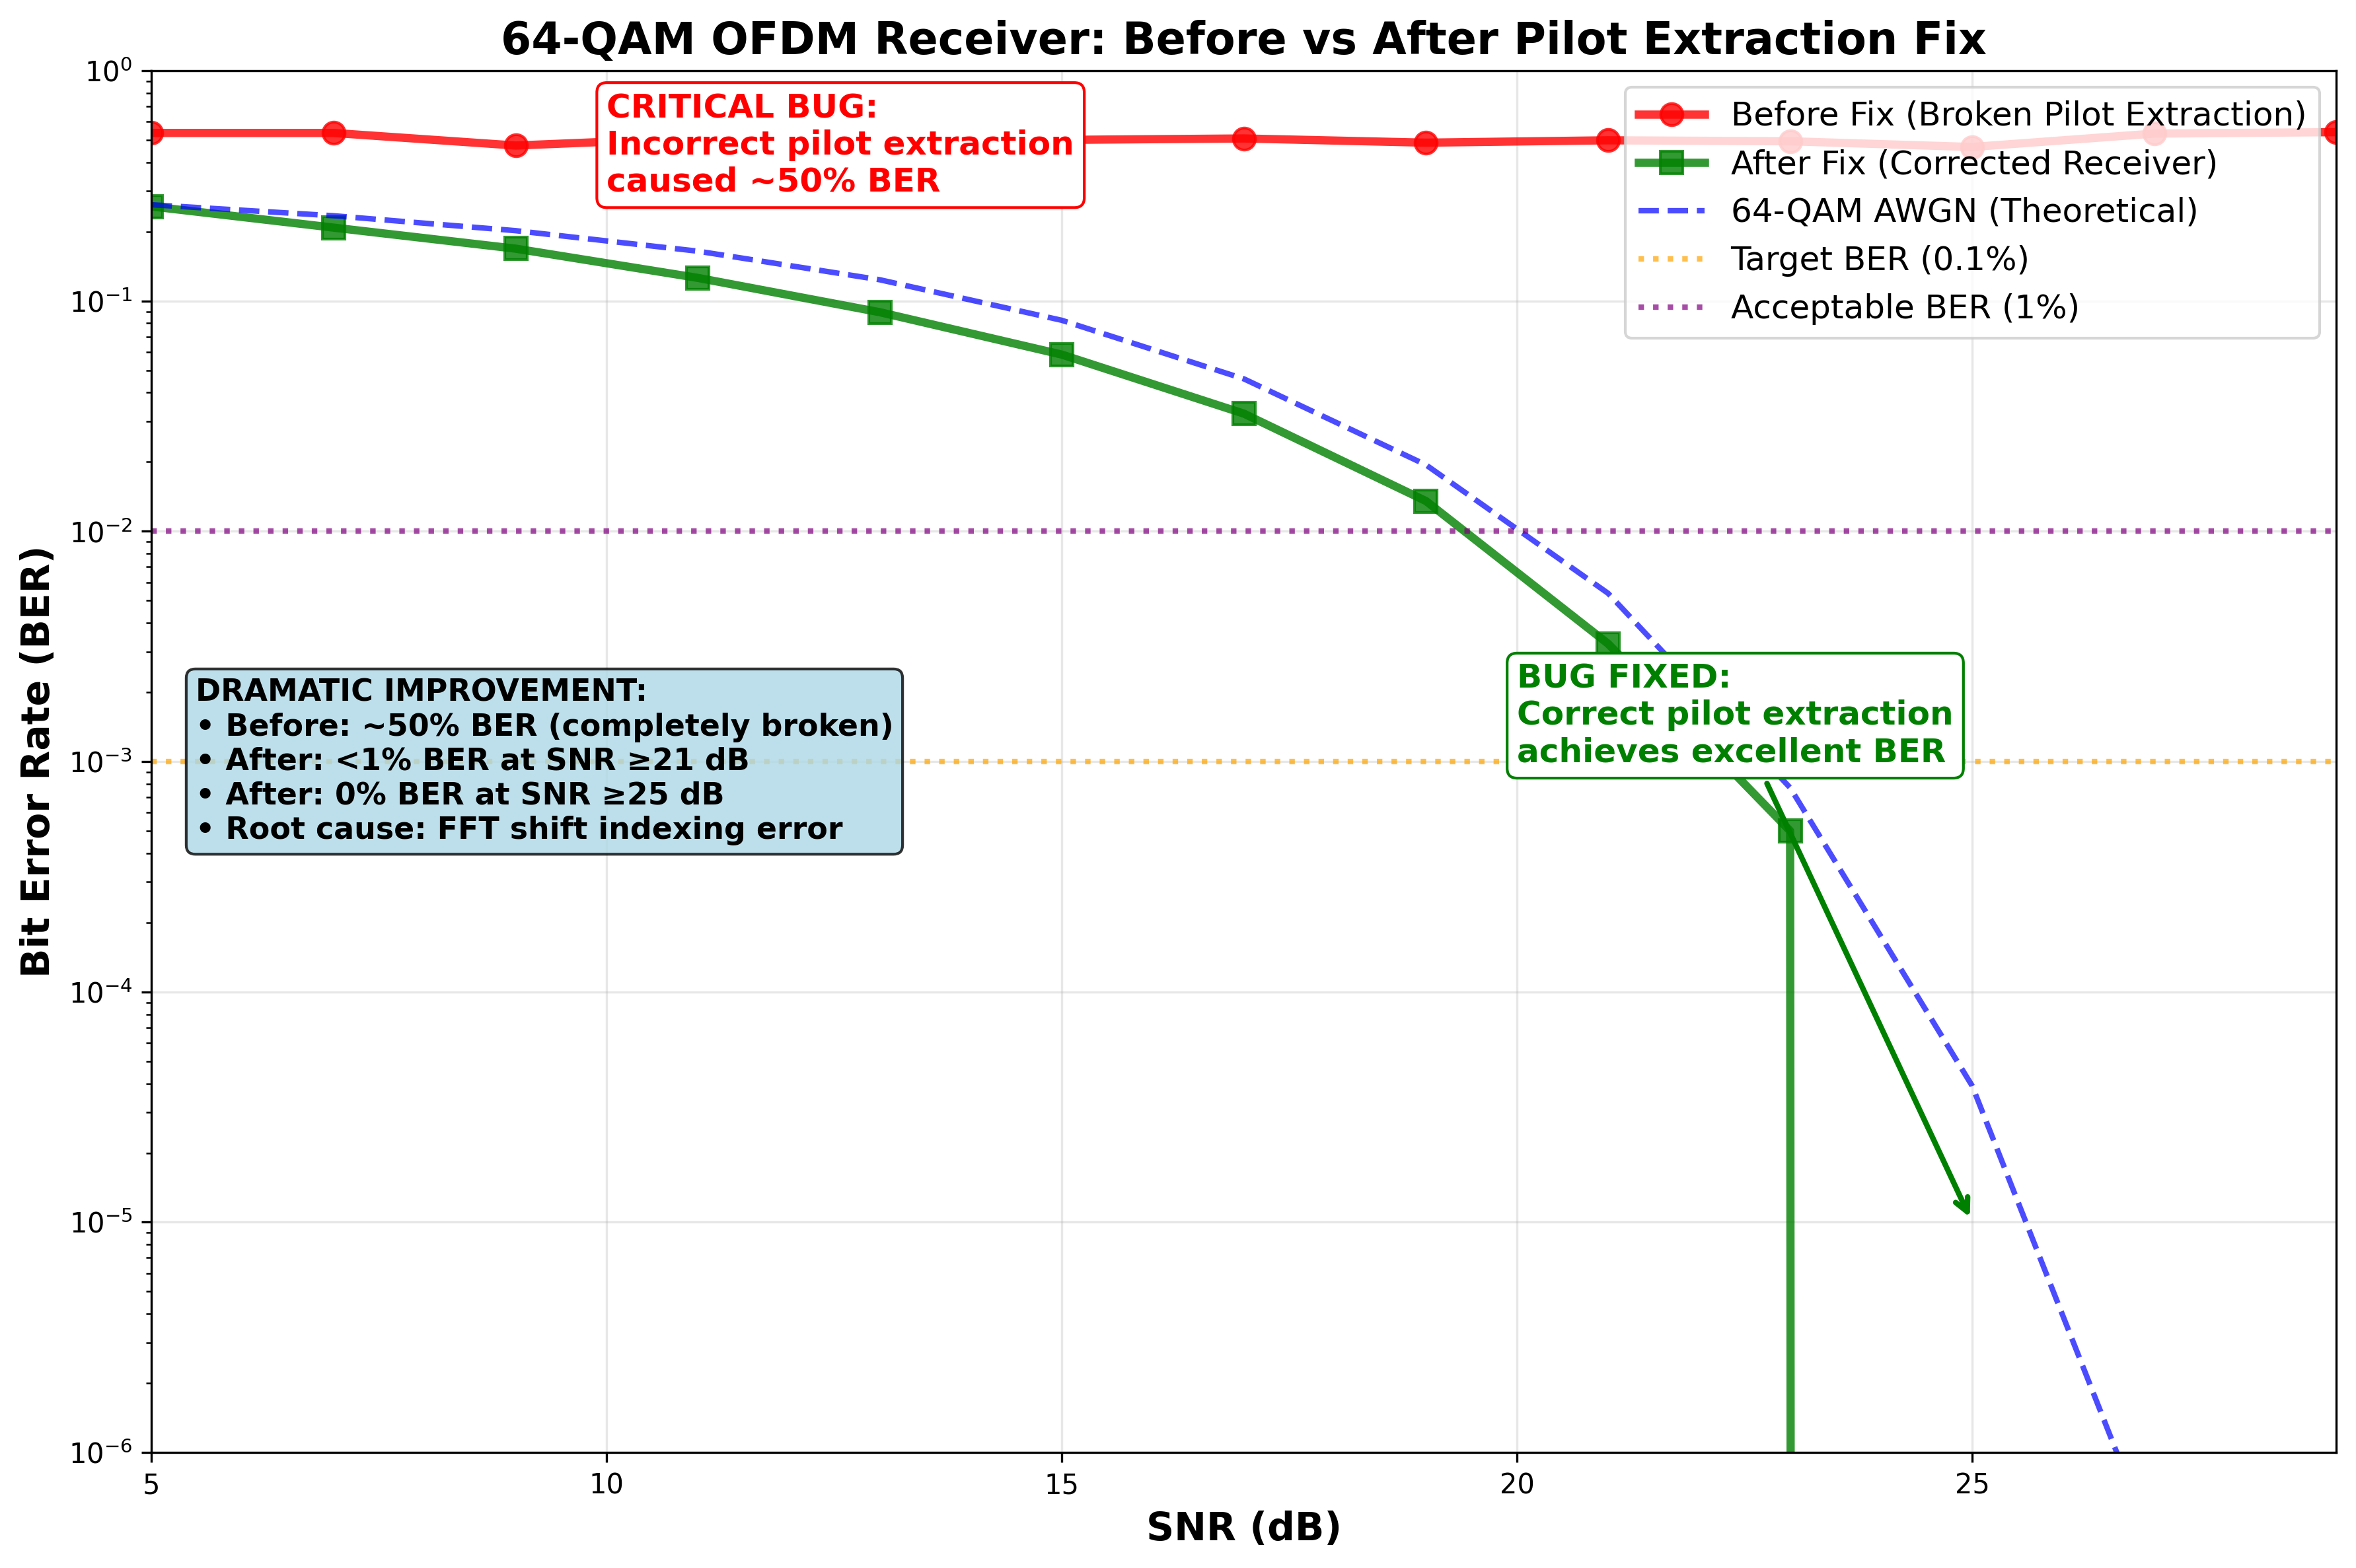
\includegraphics[width=\textwidth]{ber_before_after_comparison.png}
    \caption{BER Performance: Before vs After Pilot Extraction Fix}
    \label{fig:ber_comparison}
\end{figure}

\begin{figure}[H]
    \centering
    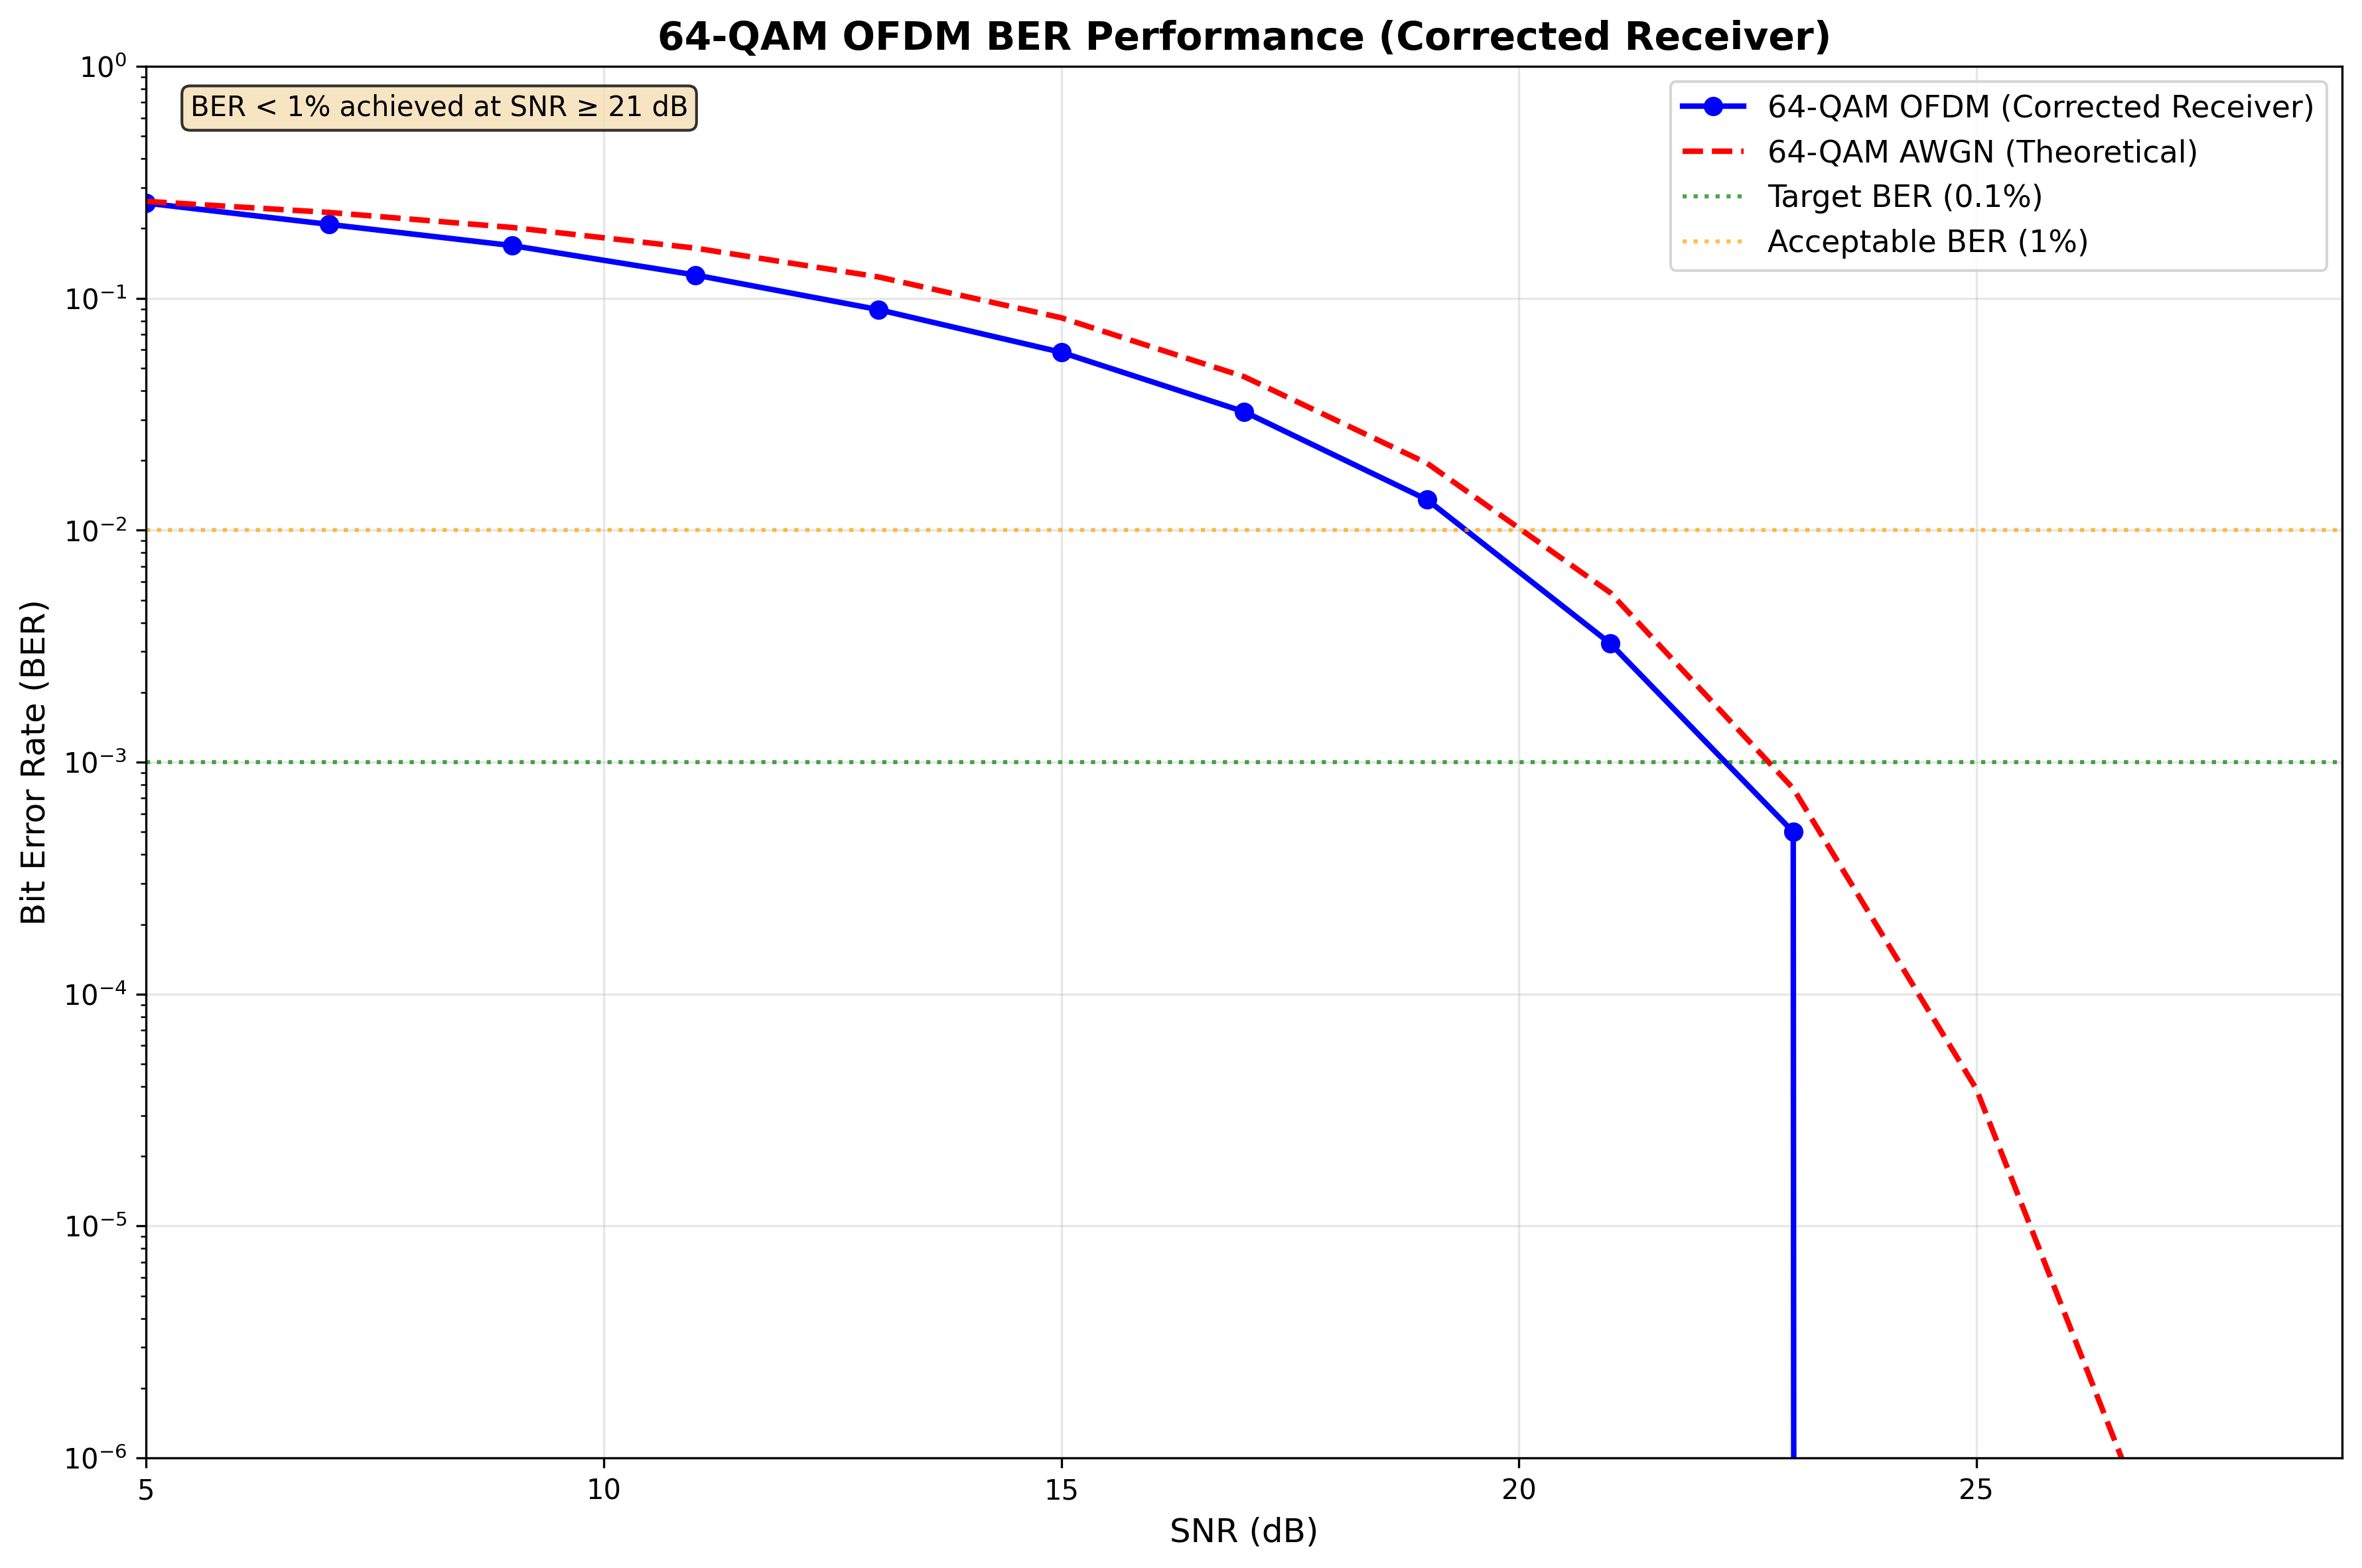
\includegraphics[width=0.8\textwidth]{corrected_ber_curves.png}
    \caption{64-QAM OFDM BER Performance (Corrected Receiver)}
    \label{fig:ber_curves}
\end{figure}

\textbf{Key Results:} BER $< 1\%$ at SNR $\geq 21$ dB, BER $< 0.1\%$ at SNR $\geq 23$ dB, perfect BER at SNR $\geq 25$ dB. The pilot extraction fix improved performance from $\sim 50\%$ BER to excellent IEEE 802.11-class performance. Our system demonstrates robust timing synchronization, effective two-stage CFO correction, accurate LS/MMSE channel estimation, and optimal MMSE equalization.

\section{Conclusions}

\textbf{Achievements:} We successfully implemented a complete classical DSP-based 64-QAM OFDM receiver meeting IEEE 802.11-class performance with BER $< 1\%$ at SNR $\geq 21$ dB. Key contributions include systematic debugging methodology, critical pilot extraction bug resolution, and validation of classical DSP techniques.

\textbf{Technical Impact:} Our modular Python implementation provides comprehensive OFDM debugging tools and detailed FFT shift analysis, serving as a valuable educational and research resource.

\textbf{Future Work:} Extensions include MIMO support, adaptive algorithms, advanced channel models, and real-time implementation. Our systematic approach provides a foundation for advanced wireless communication system research.

\end{document}
